\section{Lecture 11 (15 V 2019)}
Topic: Nash equilibrium

\begin{figure}[H]
    \centering
    \caption{A sample payoff table for 2 players and 2 strategies}
    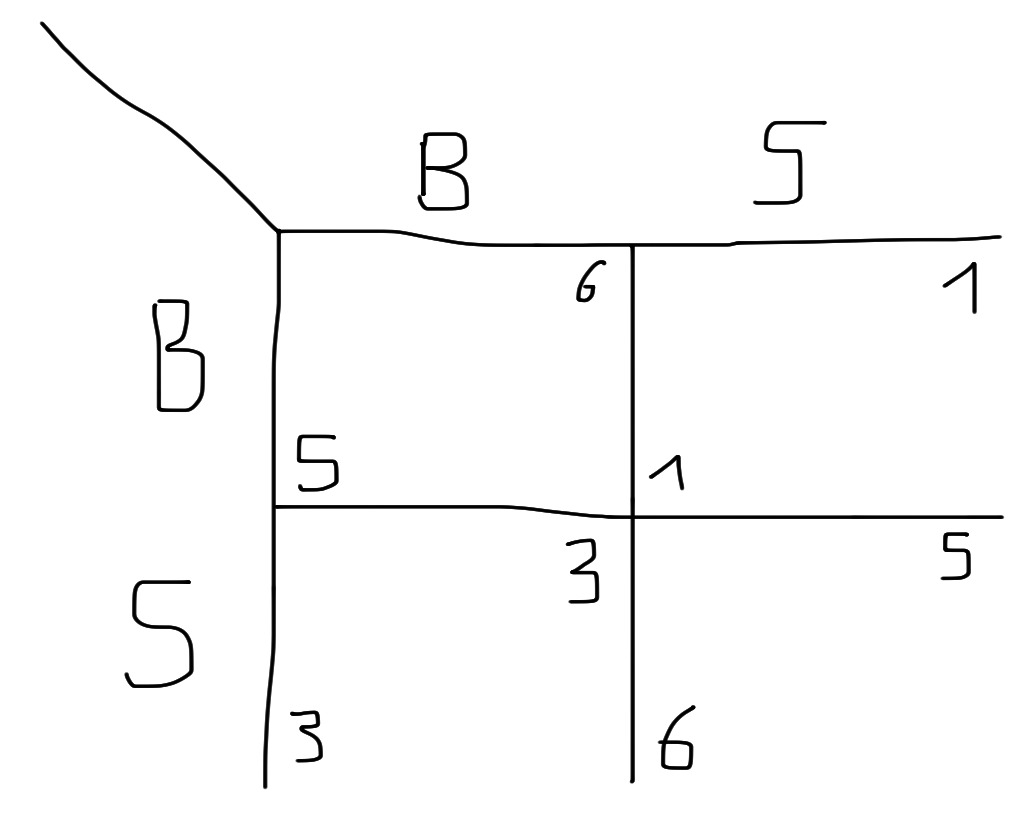
\includegraphics[scale=0.1]{content/graphics/game21.png}
\end{figure}

\noindent
$\underset{x}{sup}\ \underset{y}{inf}\ f(x, y) \stackrel{?}{\leq} \underset{y}{inf}\ \underset{x}{sup}\ f(x, y)$\\

\noindent
$\underset{y}{inf}\ f(x_0, y) \leq f(x_0, y_0) \leq \underset{x}{sup}\ f(x, y_0)$\\

\noindent
$\underset{x}{sup}\ \underset{y}{inf}\ f(x, y) \leq \underset{y}{inf}\ \underset{x}{sup}\ f(x, y)$\\

\noindent
$S_E, S_A$ -- sets of strategies for Eve and Adam\\
$f(s_E, s_A) = \begin{cases}
    1\text{, Eve wins}\\
    0\text{, Adam wins}
\end{cases}$\\

\noindent
$\underset{s_E}{sup}\ \underset{s_A}{inf}\ f(s_E, s_A) \stackrel{?}{=} \underset{s_A}{inf}\ \underset{s_E}{sup}\ f(s_E, s_A)$\\
The above equality holds if and only if the game is \textbf{determined}.\\

\noindent
\textbf{Nondeterminacy:}\\
$\forall_{s_E} \exists_{s_A} f(s_E, s_A) = 0$\\
$\forall_{s_A} \exists_{s_E} f(s_E, s_A) = 1$\\
Then:\\
$\underset{s_A}{inf}\ \underset{s_E}{sup}\ f(s_E, s_A) = 1$\\
$\underset{s_E}{sup}\ \underset{s_A}{inf}\ f(s_E, s_A) = 0$\\

\noindent
Consider the following game:\\
There is a scholarship to be granted to a single student. Let $S$ be the set of students, $P$ be the set of classes.
Each student's value is $\Theta(p, s) \cdot 100$ PLN, where $\Theta(p, s)$ is the student's grade from class $p$.
So the value of scholarship depends on the student's grade.\\
The student council chooses the student ($s$) and the financial dean chooses the class ($p$).\\
Consider variant, where both sides make their choices independently. When will neither side regret their choice?\\

\noindent
If (and only if):\\
$\underset{s}{sup}\ \underset{p}{inf}\ \Theta(s, p) = \underset{p}{inf}\ \underset{s}{sup}\ \Theta(s, p)$\\\\

\noindent
Another example: pollution game:\\
There are $N$ countries. A country which controls air pollution, pays $3$. A country which does not control air pollution,
pays $1$ to everyone.\\
Without control, everyone pays $N-1$. With control, everyone pays $3$.

\subsection*{Braess paradox}
There are two roads to get from $A$ to $B$. There are $N = 100$ people driving. The time of traversing the edge with $1$ is $1$ hour.
The time of traversing the edge with $x$ is $\frac{n}{N}$ hours, where $n$ is the number of people who have chosen this edge.
\begin{figure}[H]
    \centering
    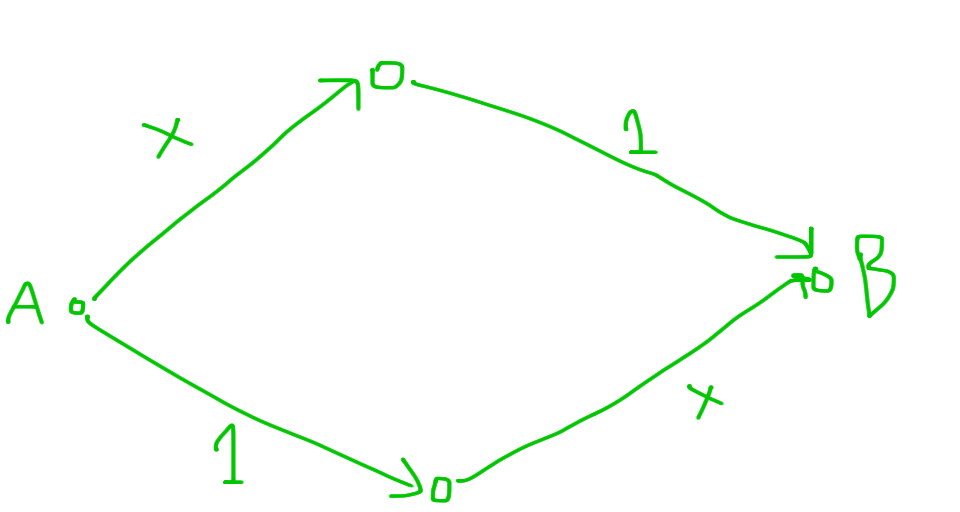
\includegraphics[scale=0.2]{content/graphics/game22.png}
\end{figure}
\noindent
The equilibrium exists -- drivers divide in two equal groups.\\
Consider what happens, when a superfast edge is added:
\begin{figure}[H]
    \centering
    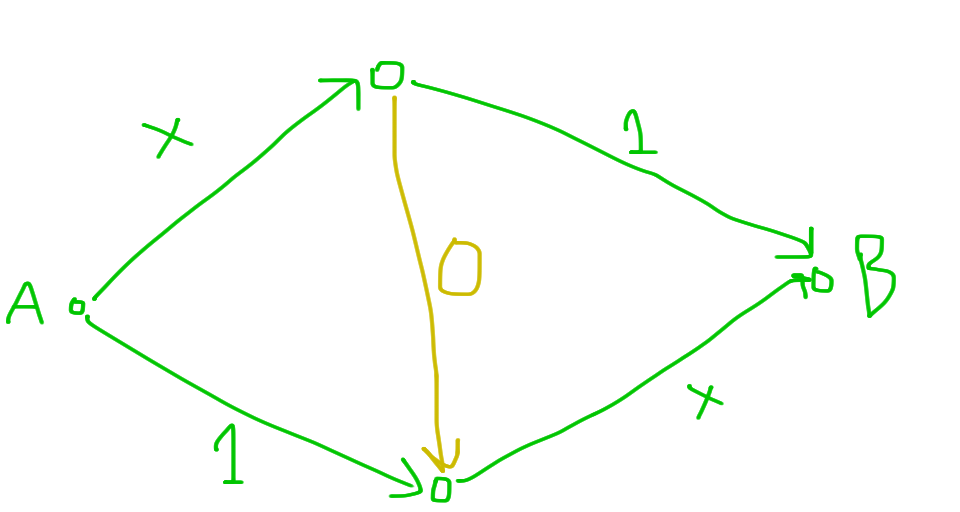
\includegraphics[scale=0.2]{content/graphics/game23.png}
\end{figure}

\subsection*{Tragedy of commons}
$N$ people want to appear on television.
\begin{figure}[H]
    \centering
    \caption{A replica of prof. Niwiński's drawing}
    
\includegraphics[scale=0.1]{content/graphics/game24.png}
\end{figure}
\noindent
$x_i$ is a time $i$-th player speaks. If $\sum_{x_i} = 1$, the player does not have time.\\
If $\sum_{x_i} < 1$, then time $i$ is $x_i (1 - \sum_{j=1}^{N} x_j)$.\\
$i$-th reasoning:\\
If $\sum_{j \neq i} x_j = t$, then maximize $-x^2 - (t-1)x$. He or she chooses $2t(t-1)$.\\
We get a set of equations:\\
$2x_1 + x_2 + x_3 + ... + x_N = 1$\\
$x_1 + 2x_2 + x_3 + ... + x_N = 1$\\
...\\
$x_1 + x_2 + x_3 + ... + 2x_N = 1$\\
Then $x_i = \frac{1}{N+1}$. $i$-th time live is $\frac{1}{(N+1)^2}$. Total time is $\frac{1}{N+1}$.
If everyone chose a smaller value, $\frac{1}{2N}$, then total time would be $\frac{1}{2}$.